% description.tex
%-----------------
\clearpage
\section{Description}
\synopsis

\begin{verbatim}
  use Chart::type;     (type is one of: Bars, Composite,
  Direction, ErrorBars, HorizontalBars, Lines, LinesPoints,
  Mountain, Pareto, Pie, Points, Split or StackedBars)

  $obj = Chart::type->new();
  $obj = Chart::type->new(\$width, \$height);

  $obj->set( $key_1,   $val_1, ... , $key_n,   $val_n);
  $obj->set( $key_1 => $val_1, ... , $key_n => $val_n);
  $obj->set( %hash );

  # Graph.pm-style API to produce PNG formatted charts:
  @data = ( \@x_tick_labels, \@dataset_1, ... , \@dataset_n);
  $obj->png( "filename", \@data );
  $obj->png( $filehandle, \@data );
  $obj->png( FILEHANDLE, \@data );
  $obj->cgi_png();

  # Graph.pm-style API:
  $obj->add_pt($label, $val_1, ..., $val_n);
  $obj->add_dataset($val_1, ..., $val_n);
  $obj->png("filename");
  $obj->png($filehandle);
  $obj->png(FILEHANDLE);
  $obj->cgi_png();
  # Similar functions are available for JPEG output.

  # Retrieve imagemap information:
  $obj->set('imagemap' => 'true');
  $imagemap_ref = $obj->imagemap_dump();

\end{verbatim}
\clearpage

The Perl module \class{Chart} creates \textsc{png} or \textsc{jpeg}
output which can be written to a file or to stdout. Therefore,
\class{Chart} can also create dynamic charts for web sites.

Many different chart types are available, viz., Bars,
Composite, Direction, ErrorBars, HorizontalBars, Lines, LinesPoints,
Mountain, Pareto, Pie, Points, Split, and StackedBars. Each
specific type is implemented as a class by itself which is
derived from the same abstract superclass, Base.

The hierarchy of \class{Chart} classes is shown in
Figure~\ref{fig:Aufbau}.

\begin{figure}[ht]
  \begin{center}
    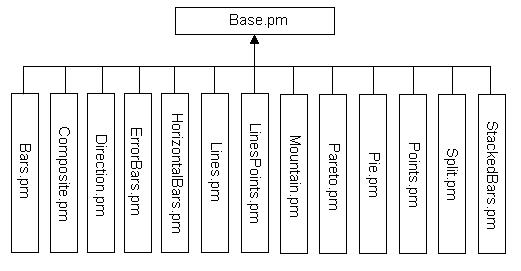
\includegraphics[scale=0.5]{Aufbau.png}
  \end{center}
  \caption{The hierarchy of \class{Chart} classes}
  \label{fig:Aufbau}
\end{figure}

You must create an \emph{instance of one of the concrete subclasses} to
get a \class{Chart} object. Take a look at the individual class
descriptions to see how they work.

All the methods and most of the options \class{Chart} provides are
implemented in the \class{Chart::Base} class. However, drawing of the
graph itself happens in the appropriate subclass.
Figure~\ref{fig:Elemente} shows the elements of a chart from a layout
perspective.

\begin{figure}[ht]
  \begin{center}
    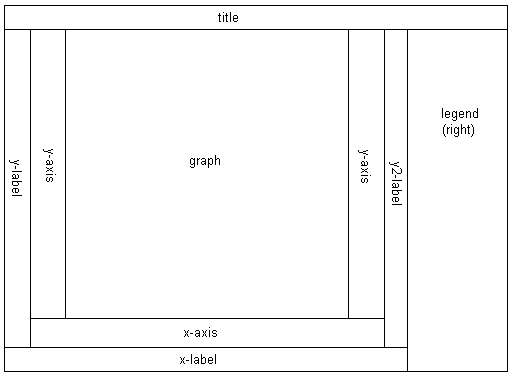
\includegraphics[scale=0.4]{Elemente.png}
  \end{center}
  \caption{Layout Elements of a chart}
  \label{fig:Elemente}
\end{figure}

The graph area in the middle is drawn by the subclass, all the other
elements are drawn by \class{Chart::Base}. But some classes do not need
all of those elements, or they may need additional elements. The
\class{Chart::Base} methods producing these elements have then to be
overwritten in the respective subclass. For example, class
\class{Chart::Pie} needs no axes, so the methods for drawing these in
file Base.pm are overwritten by methods in class \class{Chart::Pie}; in
this case, no axes are drawn. Furthermore, the legend in a pie chart is
slightly different. Therefore, Pie.pm has its own methods for drawing
the legends. All these rules are managed by \class{Chart}, so you do not
have to attend to it.

\class{Chart} uses Lincoln Stein's GD module for all its graphics
primitives calls. So you need an installed version of GD.pm to use
\class{Chart}. This module is available in the CPAN online archive at
\texttt{http://www.cpan.org/}, just like \class{Chart} itself.
\index{GD (module by Lincoln Stein)}

The table lists all attributes that are currently used within the Chart
package. It shows which of the concrete subclasses uses each attribute.

{
\begin{sidewaystable}
\tiny
\begin{tabular}{|l|c|c|c|c|c|c|c|c|c|c|c|c|c|}
\hline
Attribute & Bars& Composite& Direction& ErrorBars& HorizontalBars& Lines& LinesPoints& Mountain& Pareto& Pie& Points& Split& StackedBars \\
\hline
angle\_interval        &   &   & X &   &   &   &   &   &   &   &   &   &   \\
arrow                  &   &   & X &   &   &   &   &   &   &   &   &   &   \\
brush\_size            &   &   & X & X &   & X & X &   &   &   &   &   &   \\
brush\_size1           &   & X &   &   &   &   &   &   &   &   &   &   &   \\
brush\_size2           &   & X &   &   &   &   &   &   &   &   &   &   &   \\
brushStyle             &   &   &   &   &   &   & X &   &   &   & X &   &   \\
brushStyle1            &   & X &   &   &   &   &   &   &   &   &   &   &   \\
brushStyle2            &   & X &   &   &   &   &   &   &   &   &   &   &   \\
colors                 & X & X & X & X & X & X & X & X & X & X & X & X & X \\
composite\_info        &   & X &   &   &   &   &   &   &   &   &   &   &   \\
custom\_x\_ticks       & X & X & X & X & X & X & X & X & X & X & X & X & X \\
f\_x\_tick             & X & X & X & X & X & X & X & X & X & X & X & X & X \\
f\_y\_tick             & X & X & X & X & X & X & X & X & X & X & X & X & X \\
f\_y\_tick1            &   & X &   &   &   &   &   &   &   &   &   &   &   \\
f\_y\_tick2            &   & X &   &   &   &   &   &   &   &   &   &   &   \\
graph\_border          & X & X & X & X & X & X & X & X & X & X & X & X & X \\
grey\_background       & X & X & X & X & X & X & X & X & X & X & X & X & X \\
grid\_lines            & X & X & X & X & X & X & X & X & X & X & X & X & X \\
imagemap               & X & X & X & X & X & X & X & X & X & X & X & X & X \\
include\_zero          & X & X & X & X & X & X & X & X & X & X & X & X & X \\
integer\_ticks\_only   & X & X & X & X & X & X & X & X & X & X & X & X & X \\
interval               &   &   &   &   &   &   &   &   &   &   &   & X &   \\
interval\_ticks        &   &   &   &   &   &   &   &   &   &   &   & X &   \\
label\_font            & X & X & X & X & X & X & X & X & X & X & X & X & X \\
label\_values          &   &   &   &   &   &   &   &   &   & X &   &   &   \\
legend                 & X & X & X & X & X & X & X & X & X & X & X & X & X \\
legend\_example\_height&   & X &   &   &   &   &   &   &   &   &   &   &   \\
legend\_example\_size  & X & X & X & X & X & X & X & X & X & X & X & X & X \\
legend\_font           & X & X & X & X & X & X & X & X & X & X & X & X & X \\
legend\_label\_values  &   &   &   &   &   &   &   &   &   & X &   &   &   \\
legend\_labels         & X & X & X & X & X & X & X & X & X & X & X & X & X \\
legend\_lines          &   &   &   &   &   &   &   &   &   & X &   &   &   \\
line                   &   &   & X &   &   &   &   &   &   &   &   &   &   \\
max\_circles           &   &   & X &   &   &   &   &   &   &   &   &   &   \\
max\_val               & X & X & X & X & X & X & X & X & X & X & X & X & X \\
max\_val1              &   & X &   &   &   &   &   &   &   &   &   &   &   \\
max\_val2              &   & X &   &   &   &   &   &   &   &   &   &   &   \\
max\_x\_ticks          & X & X & X & X & X & X & X & X & X & X & X & X & X \\
max\_y\_ticks          & X & X & X & X & X & X & X & X & X & X & X & X & X \\
min\_circles           &   &   & X &   &   &   &   &   &   &   &   &   &   \\
min\_val               & X & X & X & X & X & X & X & X & X & X & X & X & X \\
min\_val1              &   & X &   &   &   &   &   &   &   &   &   &   &   \\
min\_val2              &   & X &   &   &   &   &   &   &   &   &   &   &   \\
min\_x\_ticks          & X & X & X & X & X & X & X & X & X & X & X & X & X \\
min\_y\_ticks          & X & X & X & X & X & X & X & X & X & X & X & X & X \\
no\_cache              & X & X & X & X & X & X & X & X & X & X & X & X & X \\
pairs                  &   &   & X &   &   &   &   &   &   &   &   &   &   \\
png\_border            & X & X & X & X & X & X & X & X & X & X & X & X & X \\
point                  &   &   & X &   &   &   &   &   &   &   &   &   &   \\
precision              & X & X & X & X & X & X & X & X & X & X & X & X & X \\
pt\_size               &   &   & X & X &   &   & X &   &   &   & X &   &   \\
ring                   &   &   &   &   &   &   &   &   &   & X &   &   &   \\
same\_error            &   &   &   & X &   &   &   &   &   &   &   &   &   \\
same\_y\_axes          &   & X &   &   &   &   &   &   &   &   &   &   &   \\
scale                  &   &   &   &   &   &   &   &   &   &   &   & X &   \\
skip\_int\_ticks       & X & X & X & X & X & X & X & X & X & X & X & X & X \\
skip\_x\_ticks         & X & X & X & X & X & X & X & X & X & X & X & X & X \\
skip\_y\_ticks         &   &   &   &   & X &   &   &   &   &   &   &   &   \\
sort                   &   &   & X & X &   & X & X &   & X &   & X & X &   \\
spaced\_bars           & X &   &   &   & X &   &   &   & X &   &   &   & X \\
start                  &   &   &   &   &   &   &   &   &   &   &   & X &   \\
stepline               &   &   &   &   &   & X & X &   &   &   &   &   &   \\
stepline\_mode         &   &   &   &   &   & X & X &   &   &   &   &   &   \\
sub\_title             & X & X & X & X & X & X & X & X & X & X & X & X & X \\
text\_space            & X & X & X & X & X & X & X & X & X & X & X & X & X \\
tick\_label\_font      & X & X & X & X & X & X & X & X & X & X & X & X & X \\
tick\_len              & X & X & X & X & X & X & X & X & X & X & X & X & X \\
title                  & X & X & X & X & X & X & X & X & X & X & X & X & X \\
title\_font            & X & X & X & X & X & X & X & X & X & X & X & X & X \\
transparent            & X & X & X & X & X & X & X & X & X & X & X & X & X \\
x\_grid\_lines         & X & X & X & X & X & X & X & X & X & X & X & X & X \\
x\_label               & X & X & X & X & X & X & X & X & X & X & X & X & X \\
x\_ticks               & X & X & X & X & X & X & X & X & X & X & X & X & X \\
xlabels                &   &   &   & X &   & X & X &   &   &   & X &   &   \\
xrange                 &   &   &   & X &   & X & X &   &   &   & X &   &   \\
xy\_plot               &   &   &   & X &   & X & X &   &   &   & X &   &   \\
y\_axes                & X &   &   & X & X &   & X & X & X &   & X & X & X \\
y\_grid\_lines         & X & X & X & X & X & X & X & X & X & X & X & X & X \\
y\_label               & X & X & X & X & X & X & X & X & X & X & X & X & X \\
y\_label2              & X & X & X & X & X & X & X & X & X & X & X & X & X \\
y\_ticks               & X & X & X & X & X & X & X & X & X & X & X & X & X \\
y\_ticks1              &   & X &   &   &   &   &   &   &   &   &   &   &   \\
y\_ticks2              &   & X &   &   &   &   &   &   &   &   &   &   &   \\
ylabel2                & X & X & X & X & X & X & X & X & X & X & X & X & X \\
\hline
\end{tabular}
\end{sidewaystable}
}

